%% LaTeX-Beamer template for KIT design
%% by Erik Burger, Christian Hammer
%% title picture by Klaus Krogmann
%%
%% version 2.1
%%
%% mostly compatible to KIT corporate design v2.0
%% http://intranet.kit.edu/gestaltungsrichtlinien.php
%%
%% Problems, bugs and comments to
%% burger@kit.edu

\documentclass[18pt]{beamer}

%% SLIDE FORMAT

% use 'beamerthemekit' for standard 4:3 ratio
% for widescreen slides (16:9), use 'beamerthemekitwide'

\usepackage{templates/beamerthemekit}
% \usepackage{templates/beamerthemekitwide}

%% TITLE PICTURE

% if a custom picture is to be used on the title page, copy it into the 'logos'
% directory, in the line below, replace 'mypicture' with the 
% filename (without extension) and uncomment the following line
% (picture proportions: 63 : 20 for standard, 169 : 40 for wide
% *.eps format if you use latex+dvips+ps2pdf, 
% *.jpg/*.png/*.pdf if you use pdflatex)

%\titleimage{mypicture}

%% TITLE LOGO

% for a custom logo on the front page, copy your file into the 'logos'
% directory, insert the filename in the line below and uncomment it

%\titlelogo{mylogo}

% (*.eps format if you use latex+dvips+ps2pdf,
% *.jpg/*.png/*.pdf if you use pdflatex)

%% TikZ INTEGRATION

% use these packages for PCM symbols and UML classes
% \usepackage{templates/tikzkit}
% \usepackage{templates/tikzuml}

% the presentation starts here

\title[GUI]{Dynamic scheduler for scientific simulations}
\subtitle{GUI}
\author{Kai Bittner, Ard Kastrati, Fabio Broghammer, Jan Ellmers, David Krenz, Benjamin-Philip Roth}

\institute{Steinbuch Centre for Computing (SCC)}

% Bibliography

\usepackage[citestyle=authoryear,bibstyle=numeric,hyperref,backend=biber]{biblatex}
\usepackage{tikz}
\usetikzlibrary{shapes}
 \usepackage{marvosym}
\addbibresource{templates/example.bib}
\bibhang1em

\begin{document}

% change the following line to "ngerman" for German style date and logos
\selectlanguage{english}

%title page
\begin{frame}
\titlepage
\end{frame}

%table of contents
\begin{frame}{Outline}
\tableofcontents
\end{frame}

\section{Introduction}
	\begin{frame}{Introduction}
		\begin{itemize}
			\pause
			\item The graphical user interface is an optional feature so the scientists can easily use MOAB Workload Manager and dynamic scheduler interface. 
			\pause
			\item The user can generate a shell script for MOAB Workload Manager and send it via SSH to the server.
			\pause
			\item User can also discover relationships in his/her tasks and observe the performance the program. 
			
		\end{itemize}
	\end{frame}
	
\section{Architecture}
	\begin{frame}{Architecture}
		\begin{itemize}
			\item The main architecture pattern, the graphical user interface is oriented to, is the Model-View-
Presenter. 
	        \item The view of the user interface is developed in the FXML scripting language and Java code is used for application logic.
	        
				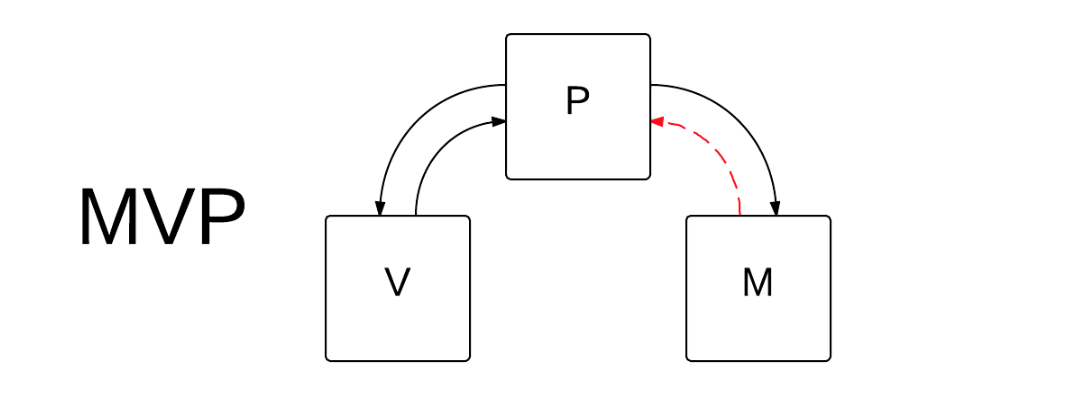
\includegraphics[width=300px, height=100px]{images/mvp.png}
		\end{itemize}
	\end{frame}
	
	
	
%	\subsection{Design}
%	\begin{frame}{Architecture (Design)}
%		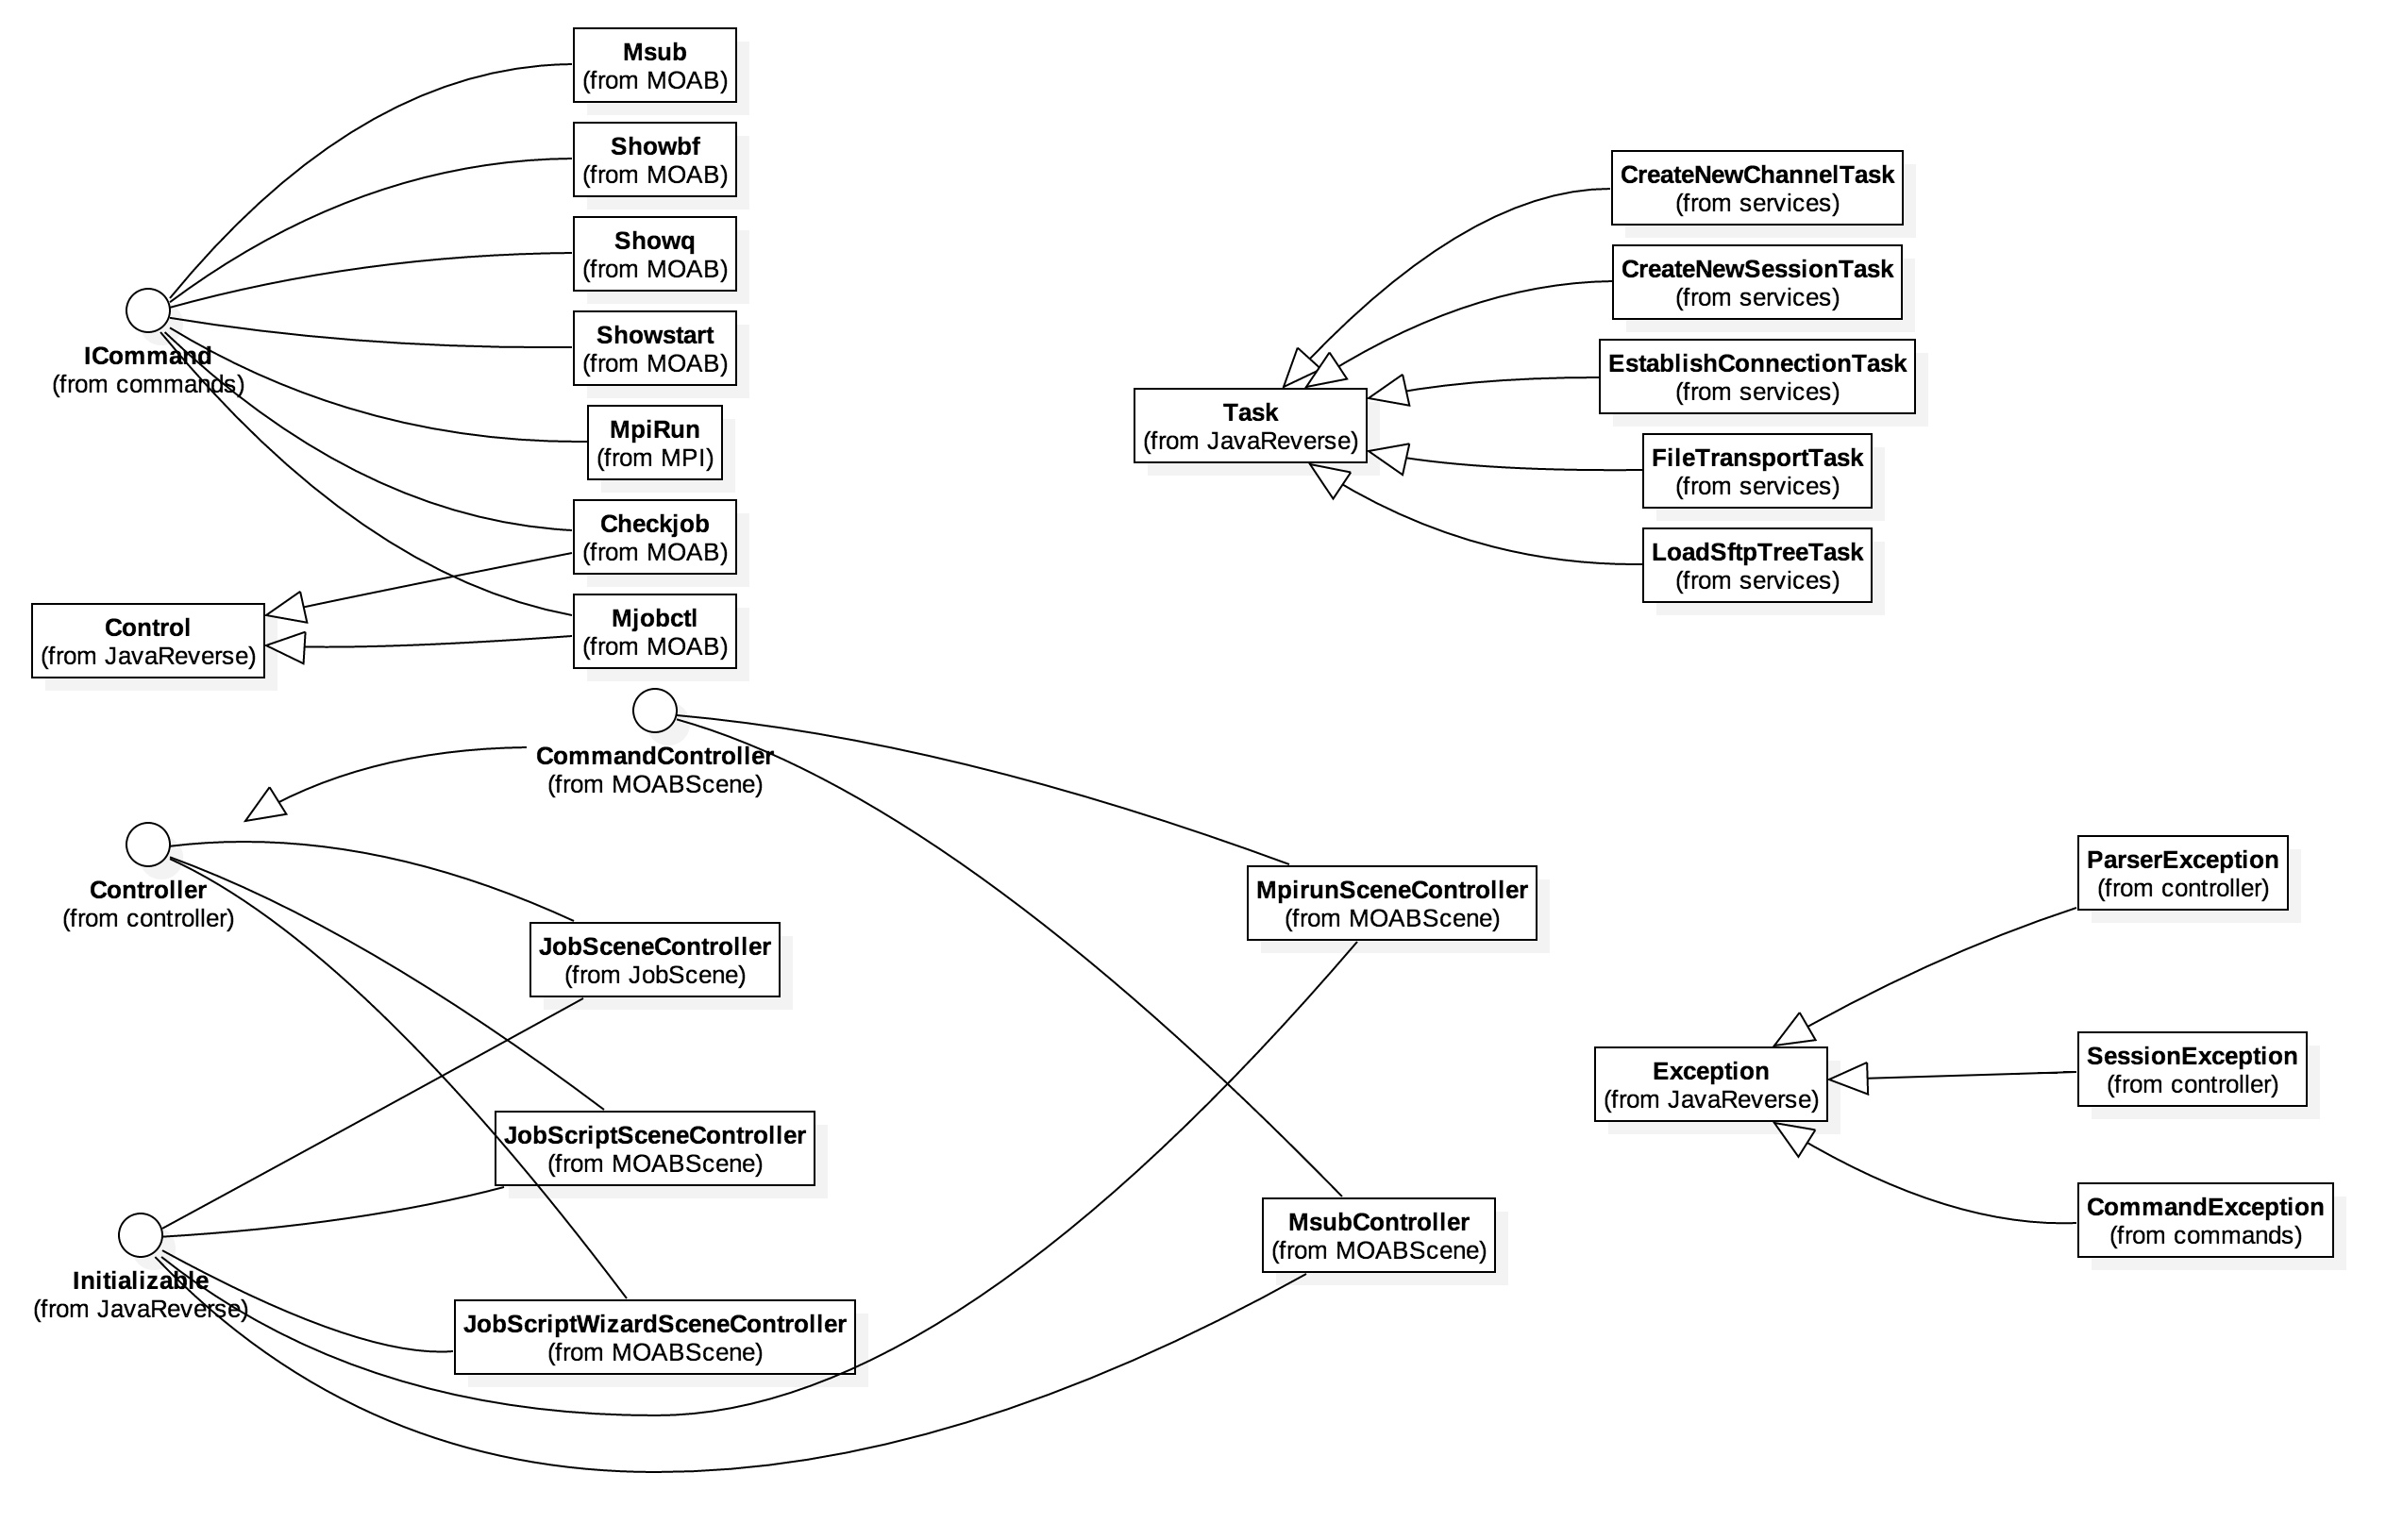
\includegraphics[width=300px, height=210px]{images/GUIDesign.png}
%	\end{frame}
	

\section{SSH-Connection}
	\begin{frame}{SSH-Connection}
		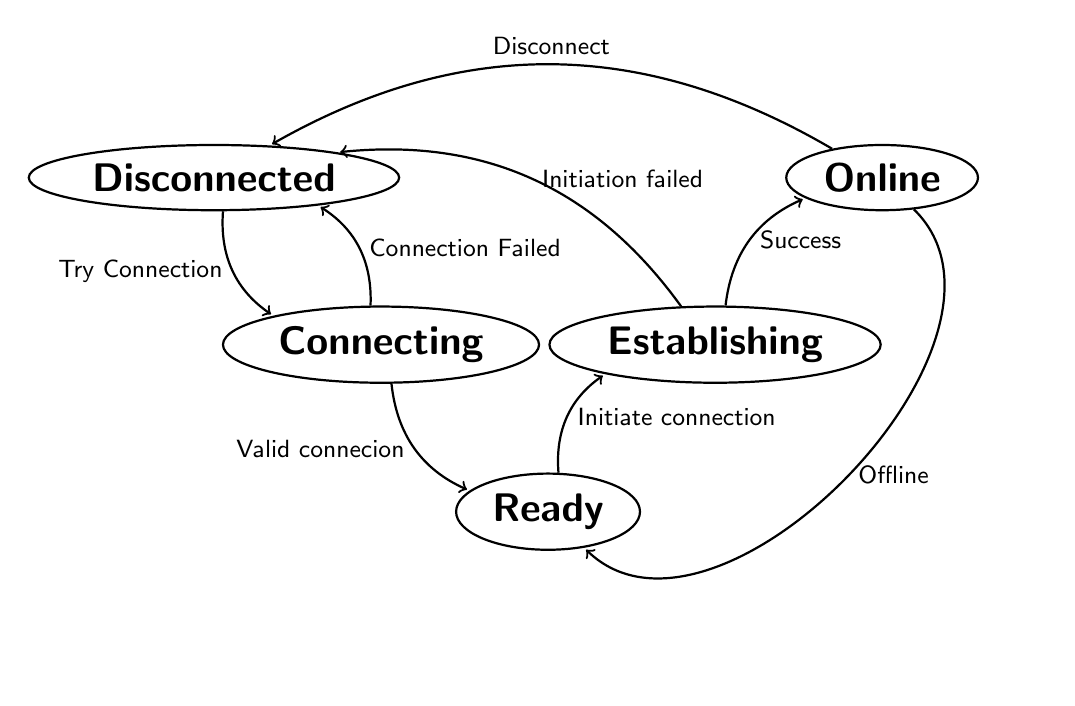
\begin{tikzpicture}[->,shorten >=1pt,auto,node distance=3cm,thick,main node/.style={ ellipse,draw,font=\sffamily\Large\bfseries}]
 
  \node[main node] (1) {Disconnected};
  \node[main node] (2) [below right of=1]{Connecting};
  \node[main node] (3) [below right of=2] {Ready};
  \node[main node] (4) [above right of=3] {Establishing};
  \node[main node] (5) [above right of=4] {Online};

  \path[every node/.style={font=\sffamily\small}]
    (1) edge [bend right] node[left] {Try Connection} (2)
        
    (2) edge [bend right] node[right] {Connection Failed} (1)
        edge [bend right] node[left] {Valid connecion} (3)
    (3) edge [bend left] node[right] {Initiate connection} (4)
    		
    (4) edge [bend right] node[right] {Initiation failed} (1)
       	edge [bend left] node[right] {Success} (5)
    (5)  edge [bend right] node[above] {Disconnect} (1)
         edge [bend left=90] node[right] {Offline} (3);
	\end{tikzpicture}
	\end{frame}
	
\section{Script generator}
	\begin{frame}{Script generator}
		Shell script generator for MOAB Workload Manager:
		
		\begin{itemize}
			\pause
			\item Parses msub command
			
			\pause			
			\item Specifies the directory in server using lazy tree 
			 
			\pause
			\item Parses mpirun command
			
			\pause
			\item Parses parameters of the dynamic scheduler
		\end{itemize}
	\end{frame}
	
	
	
	\begin{frame}{Script generator (Structure)}
		
		\begin{block}{run\_scheduler.sh}
		        \#\#\#\# MOAB commands
		        \newline
		        \newline
				\#MSUB  -q develop\\
				\#MSUB  -l nodes=22:ppn=22\\
				\#MSUB  -l walltime=1000\\
				\#MSUB  -M uxdok@student.kit.edu
				\newline
				\newline
        				\#\#\#\# Directory
				\newline
				\newline
				cd ./Documents
				\newline
				\newline
        				\#\#\#\# MPI commands
        			\newline
        			\newline
				mpirun -np 4 ./myExec -design master-worker -strategy fifo
			
		\end{block}
	\end{frame}

\section{Outcome}
	
	
\begin{frame}{Outcome}
\begin{itemize}
\item What can we do in the graphical user interface?	
\begin{itemize}
			\pause
			 \item Generate scripts and send them in the server
			 \item Visualize the performance of the program 
			 \item Discover relationships in tasks
\end{itemize}
\pause
\item GUI features are bound to the dynamic scheduler!
\pause
\item  \Frowny{} We are limited to a lot of other great MOAB Workload Manager features
%\begin{itemize}
			
%\item In The Beginning... was the Command Line - Neal Stephenson
%\end{itemize}
\pause
\item \Smiley{} Extensibility - implementation takes future growth into consideration 
	\end{itemize}
		
	\end{frame}
	
	
	
\section{Live Demo}
	
	
	\begin{frame}
		\begin{center}
			Live Demo
		\end{center}		
	\end{frame}
	
\end{document}
